\documentclass[aps,prb,twocolumn,letterpaper,twoside,nobalancelastpage,groupedaddress,amsmath,amssymb,floatfix,citeautoscript]{revtex4-1}
%\usepackage{geometry}       
%\geometry{letterpaper}     
%\usepackage[parfill]{parskip}    % Activate to begin paragraphs with an empty line rather than an indent
\usepackage{graphicx}
\usepackage{bm} %bold math symbols
\usepackage{times}
\usepackage{graphicx}
\usepackage{physics}≥
\usepackage{outlines}             
\usepackage{amssymb}
\usepackage[caption=false]{subfig}
\usepackage{mathtools}
\usepackage{color}
\definecolor{darkred}{rgb}{0.6,0.,0.}
\definecolor{darkgreen}{rgb}{0.,0.5,0.}
\definecolor{darkblue}{rgb}{0.,0.,0.6}

\usepackage{framed}

%\usepackage[square,numbers,sort,merge]{natbib}
\usepackage[
breaklinks,
colorlinks=true,
linkcolor=darkred,
citecolor=darkgreen,
urlcolor=darkblue]{hyperref}
%\usepackage{doi}

% \DeclareMathOperator{\tr}{tr}
% \DeclareMathOperator{\erf}{Erf}

\DeclareGraphicsRule{.tif}{png}{.png}{`convert #1 `dirname #1`/`basename #1 .tif`.png}

\begin{document}


\def \Ns {\mathbb{N}}
\def \Rs {\mathbb{R}}
\def \Zs {\mathbb{Z}}
\def \Qs {\mathbb{Q}}
\def \Cs {\mathbb{C}}
\def \id {\mathbb{I}}

\def \bfq {{\bf q}}
\def \bfp {{\bf p}}
\def \bfx {{\bf x}}
\def \bfy {{\bf y}}
\def \bfz {{\bf z}}
\def \bfr {{\bf r}}
\def \bfk {{\bf k}}
\def \bfn {{\bf n}}
\def \bfb {{\bf b}}
\def \bfm {\mathbf{m}}
\def \bfn {\mathbf{n}}

%\def \hata {{a}}
%\def \hatadag {{a}^{\dagger}}

\def \hatq {\widehat{q}}
\def \hatp {\widehat{p}}
\def \hata {\widehat{a}}
\def \hatadag {\widehat{a}^{\dagger}}
%\def \hatb {\widehat{b}^\phantom{\dagger}}
%\def \hatbdag {\widehat{b}^{\dagger}}
\def \wtN {\widetilde{N}}

\def \ve {\varepsilon}
\def \vth {\vartheta}



\title{Chern band geometry and the quantum Hall effect without rotational symmetry}
\author{David Bauer}
\email{dbauer@physics.ucla.edu}
\affiliation{Department of Physics and Astronomy, University of California at Los Angeles, 475 Portola Plaza, Los Angeles, California 90095, USA}

\author{Fenner Harper}
\affiliation{Department of Physics and Astronomy, University of California at Los Angeles, 475 Portola Plaza, Los Angeles, California 90095, USA}

\author{Rahul Roy}
\affiliation{Department of Physics and Astronomy, University of California at Los Angeles, 475 Portola Plaza, Los Angeles, California 90095, USA}

\date{\today}
\begin{abstract}
Abstract goes here.
 
\end{abstract}

% \pacs{0}

\maketitle

\section{Introduction}
The incompressible liquid phases of the fractional quantum Hall effect (FQHE) serve as prototypical examples of topologically ordered or gapped quantum liquid phases\cite{yoshioka_quantum_2002,fradkin_field_2013} in 2+1 dimensions. These phases are characterized by their long-range entanglement structure, which gives rise to topological quasiparticles and universal, quantized linear responses. Theoretical models of the quantum Hall (QH) fluid -- based, for example, on model wavefunctions \cite{laughlin_anomalous_1983} -- often make the simplifying assumption that the microscopic constitutent particles occupy states in a single Landau level. Some properties of Landau levels, such as nonzero Chern number \cite{thouless_quantized_1982}, are essential for the QHE, but recent work points to a need to understand the QHE in the case that the single-particle states are not Landau levels.

Among such work is the observation, due to Haldane, that the FQH fluid carries an emergent geometrical degree of freedom\cite{haldane_geometrical_2011} corresponding to the shape of elementary composite particles or `droplets.' \cite{johri_probing_2016} The geometry of the FQH fluid manifests in part as universal contributions to linear responses corresponding to perturbative variations in geometry, of which the Hall viscosity\cite{avron_viscosity_1995,tokatly_lorentz_2007,read_non-abelian_2009,haldane_hall_2009} is an example. In topological fluids, the Hall viscosity has a universal part proportional to the topological spin of the fluid\cite{read_non-abelian_2009}, which is related to the composite droplet shape.\cite{johri_probing_2016}. This geometrical degree of freedom may be obscured by the introduction of non-generic symmetries to the FQH problem implicitly, via the assumption that the underlying single-particle bands are Landau levels.


The study of the FQH beyond Landau levels has also been spurred by the discovery of fractional Chern insulators (FCI) -- time-reversal (TR) symmetry-breaking, fractionalized phases observed in the regime of strong lattice effects \cite{Bergholtz:2013ue,parameswaran_fractional_2013}. In this regime, the single-particle states reside in Chern bands rather than Landau levels. In this article, we study the geometry of Chern bands over the magnetic Brillouin zone (MBZ) defined by eigenstates of magnetic translations operators\cite{zak_magnetic_1964}. While this geometry is distinct from the emergent, many-body geometry of the FQH fluid, studies of FCIs have described how single-particle geometry influences the stability of many-body FQH phases through the GMP/$w_{\infty}$ algebra of band-projected density operators.\cite{Girvin:1986bu,parameswaran_fractional_2012,parameswaran_fractional_2013, roy_band_2014}. This connection is substantiated by numerical studies \cite{jackson_geometric_2015,Claassen2015,bauer_quantum_2016}, and researchers have employed it to engineer `ideally' stable FCI models \cite{Lee2017}. Chern band geometry can also be understood as the lattice analogue of the continuum, cyclotron-orbit geometry studied in Ref. \onlinecite{haldane_geometry_2015}.

 Research on the FQHE in the presence of a lattice potential did not originate with FCIs \cite{kol_fractional_1993,sorensen_fractional_2005,palmer_high-field_2006}, but FCIs redoubled interest in the subject with the promise of realizing FQH phases outside the usual 2DEG regime. The distinction between FCI models and the more traditional Harper-Hofstadter \cite{harper_general_1955,Azbel:1964tk,hofstadter_energy_nodate} models for lattice electron gasses is nominally that the former have no \textit{net} magnetic field per unit cell, as in the Haldane Chern insulator model\cite{haldane_model_1988}. From a theoretical point of view, this distinction is unecessary \cite{mcgreevy_wave_2012}, and we view FCIs simply as the limit of Harper-Hofstadter models when lattice effects are strong. 

 Experimental signatures of FCIs have been observed in a system of interacting electrons coupled to a superlattice potential generated in a bilayer graphene heterostructure \cite{Spantoneaan8458}. The electrons in the superlattice form Harper-Hofstadter bands with non-zero Chern number. At fractional fillings corresponding to Laughlin states in the conventional FQHE, a gapped phase with fractionally-quantized Hall conductance is observed. \cite{Spantoneaan8458}. Other experimental works have identified single-particle Chern bands in the FCI regime. \cite{Jotzu2014,Aidelsburger:2014hm,Aidelsburger:2013ew}. Chern bands can be realized in periodically-driven quantum systems, called Floquet systems, and their Berry curvature engineered and measured.\cite{Flaschner1091}
 %% Examples include the Hall viscosity \ and thermal Hall conductivity or chiral central charge\cite{Luttinger1964,Kane1997,CAPPELLI2002568,Stone2012}. 

 % The body of work described above, as well as other work studying the QHE outside the Landau level regime\cite{kapit_exact_2010,simon_fractional_2015}, raises the question of which features of Landau levels in fact contribute to stable quantum Hall phases.


The study of FQH fluid geometry intersects that of FCIs in that the addition of a non-negligible lattice potential introduces additional geometric data that may break some non-generic symmetries. For example, in the case of a square lattice, $SO(2)$ rotational invariance in the coordinate plane is explicitly broken to $C_4$ lattice symmetry. From this point of view, a complete theory of the FQHE formulated as generically as possible should furnish a theory of FCI phases. Understanding how the lattice potential of FCIs affects the geometrical responses of their topological fluid states is an active research subject. \cite{shapourian_viscoelastic_2015}

We work primarily with the weak-field limit of modified Harper-Hofstadter tight-binding models\cite{harper_general_1955,Azbel:1964tk} on a square lattice. In the presence of spatial inversion symmetry, the weak-field, effective dispersion of Chern bands in these models is generically quadratic, leading to cyclotron degrees of freedom that asymptotically reproduce Landau levels\cite{Harper:2014vi,haldane_geometry_2015}. The main result of our article is the construction of a finely-tuned, tight-binding model with Chern bands that do not approach Landau levels asymptotically in the weak-field limit. That is, we construct a model that is distinct from both FCIs and the Landau level fixed point of weak-field lattice models.

% [Experimental signatures of FCIs have been observed in a system of interacting electrons coupled to a superlattice potential generated in a bilayer graphene heterostructure \cite{Spantoneaan8458}. The electrons in the superlattice form Harper-Hofstadter bands with non-zero Chern number. At fractional fillings corresponding to Laughlin states in the conventional FQHE, a gapped phase with fractionally-quantized Hall conductance is observed. \cite{Spantoneaan8458}. Other experimental works have identified single-particle Chern bands in the FCI regime. \cite{Jotzu2014,Aidelsburger:2014hm,Aidelsburger:2013ew}. Chern bands can be realized in periodically-driven quantum systems, called Floquet systems, and their Berry curvature engineered and measured.\cite{Flaschner1091}]

% In Ref \onlinecite{Haldane2015a}, the authors studied the geometry of single-electron bands in relation to QH physics. Our article deals with similar questions, but we place an emphasis on the role played by the underlying lattice. In particular, we exhbit concrete lattice models that give rise to the band structures studied in Ref \onlinecite{Haldane2015a}. This has the benefit of making the connection between the non-generic Landau orbits and FCIs more concrete. The use of the lattice is also covenient from a numerical point of view, especially since the problem of finding the single-particle eigenstates for any choice in hopping parameters is a straightforward exercise in exact diagonalization (for a finite system).

% The Girvin-MacDonald-Platzman (GMP) algebra of projected density modes, which constrains the structure of neutral collective density excitations in the FQH fluid, 

% A second development in the FQH literature is based on observations that, in spite of their topological nature, FQH liquids are also characterized by non-trivial geometrical properties, including the Hall viscosity\cite{avron_viscosity_1995,tokatly_lorentz_2007,Read2009,haldane_hall_2009} and thermal Hall conductivity or chiral central charge\cite{Luttinger1964,Kane1997,CAPPELLI2002568,Stone2012}. These universal perturbative response coefficients are geometrical in that their calculation requires introducing a spatial metric [cite].

\section{Landau levels}
\label{landau-level-review}
Since Landau levels serve as our prototype for more general Chern bands, we begin by briefly recalling some physics of Landau levels\cite{yoshioka_quantum_2002}. We study a single electron in two dimensions in the presence of a uniform, perpendicular magnetic field $B$. The single-particle hamiltonian for non-zero $B$ is
\begin{align*}
H_0 = \frac{1}{2m}\left(\pi_1^2 + \pi_2^2\right),
\end{align*}
where $\pi_a = p_a - e A_a(\mathbf{r})$ is the gauge-covariant dynamical momentum and $p_a$ is the gauge-invariant canonical momentum. The operators $H_0$, $\pi_1$ and $\pi_2$ form a three-dimensional Heisenberg Lie algebra $\mathfrak{h}$, with commutators $\comm{H_0}{\pi_1} = \comm{H_0}{\pi_2} = 0$, and $\comm{\pi_1}{\pi_2} = i\hbar^2\ell^{-2}$, where we have introduced the \textit{magnetic length} $\ell = \sqrt{\frac{\hbar}{eB}}.$

An isomorphic presentation of this algebra is obtained by defining the \textit{cyclotron position operators}
\begin{align*}
\mathcal{R}_a = \frac{\ell^2}{\hbar}\epsilon_{ab}\pi_a,
\end{align*}
with $\comm{\mathcal{R}_a}{\mathcal{R}_b} = -i\ell^2\epsilon_{ab}$. In terms of these operators, 
\begin{align*}
H_0 = \frac{\hbar^2}{2m\ell^4}\left(\mathcal{R}^2_1 + \mathcal{R}^2_2\right),
\end{align*}
and we have $\comm{H_0}{\mathcal{R}_1} = \comm{H_0}{\mathcal{R}_2} = 0$.

We then define \textit{guiding-center position operators}
\begin{align*}
R_a = r_a - \mathcal{R}_a,
\end{align*}
which obey commutation relations $\comm{R_a}{R_b} = i\ell^2 \epsilon_{ab}$ and $\comm{R_a}{\mathcal{R}_b} = 0$, the latter of which implies $\comm{H_0}{R_a} = 0$. We see that the guiding-center and cyclotron operators each form distinct Heisenberg algebras, which we label $\mathfrak{h}^{R}$ and $\mathfrak{h}^{L}$, respectively. The superscripts $R$ and $L$ distinguish the ``right-handed'' guiding center coordinates from the ``left-handed'' cyclotron coordinates. This decomposition holds in any gauge, but the specific expressions for $\mathcal{R}_a$, $R_a$, and $H_0$ in terms of the gauge-invariant positions and momenta $r_a$, $p_a$ depend on our gauge choice.

We choose to work in the Bargmann-Fock representation of $\mathfrak{h}$ familiar from the one-dimensional quantum harmonic oscillator. Separately for each set of position operators, we choose \textit{Fock operators} or ladder operators, which are complex linear combinations of the position operators satisfying
\begin{align*}
\comm{a(\boldsymbol{\mathcal{R}})}{a^{\dag}(\boldsymbol{\mathcal{R}})} &= 1, \\
\comm{b(\boldsymbol{R})}{b^{\dag}(\boldsymbol{R})} &= 1,
\end{align*}
which are valued in the complexificaiton $\mathfrak{h}\otimes \mathbf{C}$ of the respective Heisenberg algebra. These choices are equivalent to a choice of (linear) complex structures on the cyclotron and guiding-center position spaces. The permissable complex structures are parameterized by an element of the complex upper half-plane $\mathbf{H} = \left\{\tau = \tau_1 + i\tau_2 \in \mathbf{C}, \tau_2 >0\right\}$, and the corresponding Fock operators are
\begin{align}
\label{eq-fock-tau}
a_{\tau} &= \frac{1}{\sqrt{2\ell^2\tau_2}}\left(\mathcal{R}_1 - \tau\mathcal{R}_2\right),\\ \nonumber
a_{\tau}^{\dag} &= \frac{1}{\sqrt{2\ell^2\tau_2}}\left(\mathcal{R}_1 - \tau^{\ast}\mathcal{R}_2\right),
\end{align}
with analogous expressions for the elements of $\mathfrak{h}^{R}$.
% \begin{align*}
% b &= \frac{1}{\sqrt{2\ell^2\sigma_2}}\left(R_1 - \sigma^{\ast} R_2\right),\quad
% b^{\dag} = \frac{1}{\sqrt{2\ell^2\sigma_2}}\left(R_1 - \sigma R_2\right)
% \end{align*}
% The choices of Fock operators pick out distinguished states in the respective Hilbert space which satisfy $a_{\tau}\ket{0^{L}}=0$ and $b_{\tau}\ket{0^{R}}=0$. 
The natural observables in this representation are the hermitian linear combinations
\begin{align*}
X &= \frac{a + a^{\dag}}{2} = \frac{1}{\sqrt{2\ell^2}}\left(\mathcal{R}_1 - \tau_1\mathcal{R}_2\right),\\
Y &= i\frac{a- a^{\dag}}{2} = \frac{\tau_2}{\sqrt{2\ell^2}}\mathcal{R}_2
\end{align*}

% In the Bargmann-Fock representation of $\mathfrak{h}$ gives an holomorphic functions on $\mathbf{C}$ with inner product
% \begin{align*}
% \braket{\psi_1}{\psi_2} = \int d^2z\, e^{-|z|^2/2}\, \psi_1^{\ast}(z) \psi_2(z).
% \end{align*}
% The restriction to holomorphic functions is necessary because general complex functions furnish a representation of the complexification $\mathfrak{h}\otimes\mathbf{C}$ of $\mathfrak{h}$, and this representation is only unitary on a real Lie subalgebra of $\mathfrak{h}\otimes\mathbf{C}$.

The choice of complex structure is arbitrary, but there is a natural choice found by extending this representation to a representation of $\mathfrak{sl}(2,\mathbf{R})$ with generators
\begin{align*}
\Lambda_0 &= \frac{1}{2}\left(a^{\dag}a + aa^{\dag}\right)\\
\Lambda_{+} &= \frac{1}{2}\left(a^{\dag\,2} + a^{2}\right)\\
\Lambda_{-} &= -\frac{i}{2}\left(a^{\dag\,2}- a^{2}\right)\\
\end{align*}
and commutators
\begin{align*}
\comm{\Lambda_0}{\Lambda_+} &= 2i\Lambda_-\\
\comm{\Lambda_0}{\Lambda_-} &= -2i\Lambda_+\\
\comm{\Lambda_+}{\Lambda_-} &= -2i\Lambda_0.
\end{align*}
The element $\Lambda_0$ generates the rotations $SO(2)\subset SL(2,\mathbf{R})$. A generic Landau level hamiltonian
\begin{align*}
H_0 = \frac{\hbar^2}{2m\ell^4}h_{ab}\mathcal{R}_a\mathcal{R}_b,
\end{align*}
for unimodular $h$. In the spirit of Ref. \onlinecite{avron_viscosity_1995}, we parameterize $h$ by $\tau\in\mathbf{H}$:
\begin{align*}
h = \frac{1}{\tau_2}\begin{pmatrix}1&-\tau_1\\
-\tau_1&|\tau|^2.
\end{pmatrix}
\end{align*}
By choosing $a$, $a^{\dag}$ of the form (\ref{eq-fock-tau}) with the same modular parameter $\tau$ as appears in this parameterization of $h$, we obtain
\begin{align*}
H_0 = \frac{\hbar^2}{m\ell^4}\Lambda_0.
\end{align*}
That is, $H_0$ is proportional to the generator of $SO(2)$ rotations \textit{of the cyclotron coordinate plane}.  



 % The representation of the Fock operators on this space is then given by
% \begin{align*}
% a\ket{\psi^{L}} &\rightarrow \frac{d}{dw}\psi^{L}(w),\\
% a^{\dag}\ket{\psi^{L}} &\rightarrow w\psi^{L}(w),\\
% b\ket{\psi^{R}} &\rightarrow \frac{d}{dz}\psi^{L}(z),\\
% b^{\dag}\ket{\psi^{R}} &\rightarrow z\psi^{L}(z).
% \end{align*}
% The functions $\phi_n(z) = z^n/\sqrt{n!}$ for $n \in \mathbf{Z}^{\ast}$ provide a basis for the space of holomorphic functions, corresponding to the states $\ket{n} = a^{\dag n}\ket{0}/\sqrt{n!}$

We can also define coherent states $\ket{\xi}$, which are eigenstates of the $b$ operator with eigenvalue $\xi \in \mathbf{C}$: $b\ket{\xi} = \xi \ket{\xi}$. These states can be constructed in terms of the Fock representation as
\begin{align*}
\ket{\xi_{\tau}} = e^{-|\xi|^2}e^{\overline{\xi}b_{\tau}^{\dag}}\ket{0}.
\end{align*}
While it is possible to construct position eigenstates for the total position operator, once we project to a given Landau level, we freeze the mean cyclotron radius. Since the components of the guiding-center position operator do not commute, it is not possible to construct guiding-center position eigenstates. Coherent states may be considered the closest approximation to such eigenstates, in that the total uncertainty of the $x$ and $y$ guiding-center position operators is minimized, and the uncertainty is equally distributed between the coordinates,
$\mel{\xi}{(\Delta R_1)^2}{\xi} = \mel{\xi}{(\Delta R_2)^2}{\xi}$. 

While the coherent states provide a representation of the guiding center manifold of states, they do not form a basis, in that they are overcomplete and not orthogonal.
\begin{align*}
\mathbf{1} = \frac{1}{\pi}\int_{\mathbf{C}} d^2\xi\, \dyad{\xi}
\end{align*}

The uncertainty relation between the guiding-center position operators can be expressed in terms of the geometry of the projective Hilbert space on which these operators act. In particular, projective Hilbert space carries a natural symplectic form $F$ -- the Berry curvature -- and Riemannian metric $g$ -- the Fubini-Study metric\cite{provost_riemannian_1980}. We can write these forms in components as
\begin{align*}
F_{ab}(P) &= \frac{1}{2}\text{Tr}\left(R_a P R_b P - R_b P R_a P\right)\\
G_{ab}(P) &= \text{Tr}\left(\left[R_aR_b + R_bR_a\right] P\right) - \expval{R_a}\expval{R_b}, 
\end{align*}
noting that $F_{ab}$ and $G_{ab}$ are respectively antisymmetric and symmetric in their indices.
The uncertainty relation for the guiding-center position operators is
\begin{align*}
\expval{(\Delta R_a)^2}\expval{(\Delta R_b)^2} &\geq (F_{ab})^2 + (G_{ab})^2.
\end{align*}

As observed in Ref. \cite{haldane_geometry_2015}, another expression for the uncertainty relation between the guiding-center coordinates is
\begin{align*}
\bar{g}_{ab}\left[\text{Tr}\left(\left[R_aR_b + R_bR_a\right] P\right) - \expval{R_a}\expval{R_b}\right] \geq \ell^2
\end{align*}
for any unimodular metric $\bar{g}$. This uncertainty bound is saturated when $\bar{g} = g_{\tau}$ and $P$ projects onto a coherent state, $P = P_{\xi} = \dyad{\xi_{\tau}}$. Since the trace is the Fubini-Study metric $G_{ab}$ defined above, we have
\begin{align*}
g^{\tau}_{ab}G_{ab}(P_{\xi}) = \ell^2.
\end{align*}
That is, the unimodular metric of Haldane is proportional to the inverse of the Fubini-Study metric.



% Since coherent states saturate the above uncertainty bound, the Fubini-Study metric is diagonal for \textit{any} coherent state. 

% A metric on a manifold gives us a way to compute inner products in the tangent space at each point of the manifold. In the case of projective Hilbert space, the points are projectors, and the tangent space is just the space of states in Hilbert space annihilated by the projector.
% The components of the Berry curvature and Fubini-Study metric 


% \begin{align*}
% \Omega = 
% \end{align*}

% Here we have a hamiltonian $H_0 = \frac{1}{2m}\left(\pi_x^2 + \pi_y^2\right)$, with $\pi_a = m v_a$ the dynamical momentum. The operators $H_0$, $\pi_x$ and $\pi_y$ form a Heisenberg Lie algebra, with commutators $\comm{\pi_x}{\pi_y} = i\hbar e B$, $\comm{H_0}{\pi_x} = 0$ and $\comm{H_0}{\pi_y} = 0$. The hamiltonian is diagonalized by introducing Fock operators $a$, $a^{\dagger}$. There are additional operators in the problem that commute with the hamiltonian. These are the guiding-center position operators $R_a = r_a - (eB)^{-1}\varepsilon_{ab}\pi_b$ with $\comm{R_x}{R_y} = i\hbar(eB)^{-1}$. Each subspace of states with a given energy is degenerate, and the degenerate states may be labelled by a guiding-center quantum number.

\section{Tight-binding models and Chern bands}
\subsection{Effective Landau levels from weak-field Harper-Hofstadter models}
\label{landau-level-limit}
In this section, we will show that, to lowest order in magnetic flux per lattice plaquette, the effective continuum hamiltonian of a Hofstadter-type model on a two-dimensional Bravais lattice is the Landau level hamiltonian. We will assume that the hopping amplitude between any two sites on the lattice is generically non-zero. We index the sites of the lattice by a vector $\mathbf{m} = (m_1, m_2)$ with integer components. Let $c^{\dag}_{\mathbf{m}}$ ($c_{\mathbf{m}}$) create (annihilate) an electron at site $\mathbf{m}$ of the lattice. We have the usual fermion anticommutation relations $\left\{c_{\mathbf{m}},c_{\mathbf{n}}^{\dag}\right\} = \delta_{\mathbf{m} \mathbf{n}}$. The single-particle Hilbert space is spanned by the space of states $\ket{\mathbf{m}}$ with the electron occupying site $\mathbf{m}$. The hamiltonian in this representation is
\begin{align*}
H &= -\sum_{\mathbf{m}\neq \mathbf{n}} t_{\mathbf{m}\mathbf{n}} c^{\dag}_\mathbf{n} c_\mathbf{m}  + t_{\mathbf{n}\mathbf{m}} c^{\dag}_{\mathbf{m}} c_{\mathbf{n}}\\  &= \sum_{\mathbf{m}\neq \mathbf{n}} t_{\mathbf{m}\mathbf{n}} \dyad{\mathbf{n}}{\mathbf{m}} + t_{\mathbf{n}\mathbf{m}} \dyad{\mathbf{m}}{\mathbf{n}}
\end{align*}
Note that we are excluding onsite/mass terms from the above hamiltonian; this is because a translation-invariant mass term simply shifts $H$ by a constant. We define lattice translation operators $T_a = \sum_{\bfm} \dyad{\mathbf{m} + \mathbf{e}_a}{\mathbf{m}}$. We can write the hamiltonian in terms of these as
\begin{align}
\label{eq-b0-lattice-hamiltonian}
H = -\sum_{j,k} t_{jk} \left(T_1^j T_2^k + (T^{\dag}_2)^{k} (T^{\dag}_1)^{j}\right)
\end{align}
We stipulate that this hamiltonian should be time-reversal invariant in the absence of any magnetic flux, so the $t_{jk}$ will be real here and and in the following.

We introduce a uniform background magnetic field $B$ perpendicular to the spatial extent of the lattice. We choose the value of $B$ to be such that the flux per lattice plaquette is $Ba^2 = \frac{P}{Q}\phi_0$, where $\phi_0 = 2\pi \hbar /e$ is the magnetic flux quantum and $P$ and $Q$ are relatively prime integers. In terms of the magnetic length and lattice spacing, we have $a^2/\ell^2 = 2 \pi P/Q$. We now define $\varepsilon^2 \coloneqq a^2/\ell^2$. In the presence of the magnetic field, the above translation operators are no longer gauge invariant \cite{FradkinBook}. Instead, the correct lattice translation operators in this case are
\begin{align*}
\widetilde{T}_a = \sum_{\mathbf{m}} e^{i\theta_a(\mathbf{m})} \dyad{\bfm + \mathbf{e}_a}{\bfm}.
\end{align*}
where the phases $e^{i\theta_a(\bfm)}$ satisfy 
\begin{align*}
\theta_1(\bfm) + \theta_2(\bfm + \mathbf{e}_1) - \theta_1(\bfm + \mathbf{e}_2) - \theta_2(\bfm) = \varepsilon^2,
\end{align*}
or
\begin{align*}
\Delta_1\theta_2 - \Delta_2\theta_1 = \varepsilon^2.
\end{align*}
We regard the phases $\theta$ as residing on the links of the lattice, but we canonically identify $\theta_a(\mathbf{m}) = \theta(\mathbf{m},\mathbf{m}+\mathbf{e}_a)$.
The lattice translation operators $\widetilde{T}_a$ are unitary, so we can write them in terms of hermitian generators $\widetilde{T}_a = \exp\left[-i \Pi_a\right]$. The components of $\widetilde{\mathbf{T}}$ do not commute, but satisfy $\widetilde{T}_1 \widetilde{T}_2 = \exp(i\varepsilon^2) \widetilde{T}_2 \widetilde{T}_1 $. This implies the commutator
$\comm{\Pi_1}{\Pi_2} = i \varepsilon^2.$

% [Actually, it seems like it implies $\comm{\Pi_1}{\Pi_2} = i \epsilon + 2\pi i M$ for $M \in \mathbf{Z}$. I think it's probably worthwhile to keep track of the $M$, although I'm not sure of its significance. (Also I guess for the same reason the phases should really satisfy $\sum_{\square}\theta = \epsilon + 2\pi M$). Anyway, I think I'm ok to ignore this here.]

Because the $\widetilde{T}_a$ do not commute with each other, there is an ambiguity in passing from the $B=0$ hamiltonian (\ref{eq-b0-lattice-hamiltonian}) to one for $B\neq0$, which appears as a choice of phase of the (now-complex) $t_{\mathbf{m}\mathbf{n}}$. This is analogous to the ordering ambiguity in quantizing polynomials on classical phase space. For now we fix this ambiguity by making the arbitrary choice that $T_1^j T_2^k \rightarrow \widetilde{T}_1^j \widetilde{T}_2^k + \widetilde{T}_2^k\widetilde{T}_1^j$ in the presence of nonzero $B$. We could also have fixed this ambiguity by a choice of gauge for the $\theta(\mathbf{m})$. Then
\begin{align*}
H = -\sum_{j,k} t_{jk}\left(\widetilde{T}_1^j \widetilde{T}_2^k + \widetilde{T}_2^k\widetilde{T}_1^j\right) + \text{h.c.}
\end{align*}

Let us look at just the nearest-neighbor hopping hamiltonian containing only first powers of the translation operators: $H_{\text{NN}} = -t\left(T_1 + T_1^{\dag}\right) - t'\left(T_2 + T_2^{\dag}\right)$. This part of the hamiltonian requires no ordering prescription (or gauge choice). If we set $t = t'$, $H_{\text{NN}}$ is just the hamiltonian of the Hofstadter model. Since $\widetilde{T}_a = e^{-i\Pi_a}$, we can formally write $H_{\text{NN}}= -2t\cos\left(\Pi_1\right) - 2 t'\cos\left(\Pi_1\right).$ In order to make the dependence on $\varepsilon$ explicit, we rescale the $\Pi_a$ operators, defining $\varepsilon P_a = \Pi_a$, and we have the commutation relation $\comm{P_1}{P_2} = i$. Although the commutator of the $P_a$ is $O(1)$ with respect to $\varepsilon$, we can not necessarily infer that the $P_a$ are individually $O(1)$. However, in what follows we will assume this is the case. Then
\begin{align*}
H_{\text{NN}} &= -2\sum_{n=0}^{\infty}  \frac{(-1)^{n}\varepsilon^{2n}}{(2n)!} \left(t P^{2n}_1 + t'P^{2n}_2\right)\\
&= -2 + 2\varepsilon^2\frac{\left(t P^{2}_1 + t' P^{2}_2\right)}{2} +O(\varepsilon^4).
\end{align*}
Now let $t' = \alpha^2 t$, i.e., $t$ is a common hopping energy scale and $\alpha$ parameterizes anisotropy in the hopping amplitudes. Then to lowest order in $\varepsilon = a/\ell$, we have a small-$\varepsilon$ effective hamiltonian $H_{\text{eff}}= t\varepsilon^2 \left(P^{2}_1 + \alpha^2P^{2}_2\right)$. We can rewrite this in terms of momentum operators that satisfy $\comm{\pi_x}{\pi_y} = i\hbar e B$ as
\begin{align*}
H_{\text{eff}} = \frac{1}{2m_{\ast}}\left(\pi_x^2 + \pi_y^2\right),
\end{align*}
showing that our effective hamiltonian is isomorphic to the Landau level hamiltonian with effective mass $m_{\ast} = \hbar^2/(2ta^2\alpha)$. In order to recover all of the physics of Landau levels, we also need an extensively large set of commuting observables analogous to the guiding-center positions in the continuum problem. Here, this role is filled by the magnetic translation operators, which we discuss in the following section. If we consider not just nearest-neighbor but also longer range hopping terms, the details of the above argument are slightly more complicated, but we still obtain a quadratic hamiltonian to lowest order.

\subsection{Magnetic translations and magnetic Brillouin zone}
% Given a tight-binding hamiltonian as described above, we can define magnetic translation operators $\widetilde{U}_a$ that commute with the hamiltonian. 

% As in the Landau problem, we can introduce guidi 


% Like the lattice translation operators, the magnetic translation operators consist of combined translations and gauge transformations. In order for the magnetic translations to commute with the lattice translations, the associated gauge transformations must correspond to a magnetic field directed opposite the physical magnetic field. In this sense, the magnetic translations have the opposite chirality from the lattice translations.

\begin{align*}
\widetilde{U}_a = \sum_{\mathbf{m}} e^{i\chi_a(\mathbf{m})} \dyad{\bfm + \mathbf{e}_a}{\bfm}.
\end{align*}
In order for the lattice and guiding-center translations to commute, the guiding-center gauge fluxes $\chi_a$ must satisfy
\begin{align*}
\Delta_a \theta_b = \Delta_b\chi_a,
\end{align*}
which implies
\begin{align*}
\Delta_1\chi_2 - \Delta_2 \chi_1 = -\varepsilon^2.
\end{align*}
The minus sign on the right-hand sign shows that lattice translations $\widetilde{T}_a$ and guiding-center translations $\widetilde{U}_a$ carry opposite handedness, precisely in analogy with the opposite handedness implied by the commutators $\comm{R_a}{R_b} = i\ell^2 \epsilon_{ab}$ and $\comm{\mathcal{R}_a}{\mathcal{R}_b} = -i\ell^2 \epsilon_{ab}$ of the Landau level problem.

We also define a \textit{magnetic unit cell} (MUC) containing $m \times n$ lattice sites, where $m$ and $n$ are chosen such that the MUC contains an integer number of flux quanta. Magnetic translations by one MUC commute, i.e. $\widetilde{U}_1^{m}\widetilde{U}_2^{n} = \widetilde{U}_2^{n}\widetilde{U}_2^{m}$. Since $\widetilde{U}_1$ and $\widetilde{U}_2$ commute with the hamiltonian, we can define their common eigenstates. This gives a ``guiding-center lattice'' of magnetic unit cells, each of which carries an internal Hilbert space corresponding to the cyclotron degrees of freedom.

We can define the simulatenous eigenstates of the hamiltonian and MUC translations $\ket{n,\bfk}$, where $\bfk$ takes values in the magnetic Brillouin zone and $n$ labels eigenstates of $H$. We can write the hamiltonian 
\begin{align}
\label{band-projector-ham}
H = \sum_{n}\int d^2k\, E_{n}(\bfk) P_{n,\bfk},
\end{align}
where $E_n$ is the dispersion of the $n$-th band of the hamiltonian, and $P_{n,\bfk}$ is the projector onto the state $\ket{n,\bfk}$.

 % If we work on a finite system of size $L_x \times L_y$ with periodic boundary conditions, then the dimension $d = L_x L_y$ of our Hilbert space will be finite, and the MBZ will consist of a discrete lattice in $\mathbf{k}$-space. The integral in (\ref{band-projector-ham}) will then be a finite sum; in the thermodynamic limit, the sum is replaced by an integral.
\subsection{Chern band geometry and FQHE stability}
Unlike in Landau levels, the dispersion $E_{n}(\bfk)$ generically has some finite width, and the states in the band are not exactly degenerate. In the weak-field case this bandwidth will be exponentially small\cite{Harper:2014vi}, while in the strong-field limit we may follow the usual procedure of adding long-range hoppings to flatten the band. \cite{Bergholtz:2013ue,parameswaran_fractional_2013} In either case, we will neglect the bandwidth. Despite being dispersionless, these Chern bands are distinct from Landau levels. We can quantify this distinction by considering the Berry curvature and Fubini-Study (FS) metric defined on the magnetic Brillouin zone\cite{parameswaran_fractional_2013,roy_band_2014,Claassen2015}. (The FS metric has also been called the Bures metric in this context.\cite{palumbo_momentum-space_2017}) For notational simplicity, we define $\partial_a \coloneqq \partial_{k_a}$. Then, respectively, the Berry curvature and FS metric components are 
\begin{align*}
B(\bfk) = \epsilon_{ab}\text{Tr}\left(\partial_{a}P\partial_b P\right),
\end{align*}
and
\begin{align*}
g_{ab}(\bfk) = \frac{1}{2}\text{Tr}\left(\partial_{a}Q\partial_{b}P + \partial_{b}Q\partial_{a} P\right). \\
%\left. \quad\quad-P_{n,\bfk}\left[\partial_aP_{n,\bfk}\partial_b+ \partial_bP_{n,\bfk}\partial_a\right] P_{n,\bfk}\right)
\end{align*}
The TR-symmetry breaking Chern bands that we want to study are those with nonvanishing first Chern number 
\begin{align*}
c_1 = \int d^2k\, B(\mathbf{k}).
\end{align*}

The Fubini-Study metric and Berry curvature for each band satisfy the inequalities\cite{roy_band_2014}
\begin{align*}
\left(\text{Tr}\,g(\mathbf{k})\right)&\geq|B(\mathbf{k})| \\
4\left(\text{Det}\,g(\mathbf{k})\right)&\geq|B(\mathbf{k})|^2 
\end{align*}
at every point in the MBZ.

% We denote the average of $T(\bfk)$ over the MBZ
% \begin{align*}
% \expval{T} = \frac{1}{V_{\text{MBZ}}}\int d^2k\, T_n(\bfk),
% \end{align*}
% with $V_{\text{MBZ}}$ the area of MBZ. 

To study the fractional quantum Hall effect, consider a repulsive, two-body potential on the lattice.


By consideration of the algebra of density operators projected to Chern bands -- the analogue of the well-known Girvin-MacDonald-Platzmann (GMP) algebra of the FQHE \cite{Girvin:1986bu} -- one can infer quantative measures of deviations from ``ideal'' LL behavior\cite{parameswaran_fractional_2012,roy_band_2014}. Specifically, if the Berry curvature and Fubini-Study metric are uniform over the MBZ, then the algebra of projected density operators closes to $O(k^3)$. If, additionally, $T(k)=0$, this algebra closes to all orders in $k$. This suggests a connection between these geometric observables and the stability of the many-body gapped liquid phase in FCIs. Numerical evidence in both Chern insulator\cite{jackson_geometric_2015} and Harper-Hofstadter\cite{bauer_quantum_2016} regimes supports this connection.

% Recently, a possible low-energy, geometrical theory of the gapped collective mode (the GMP mode) has been developed. In this theory, a quantity analogous to 

The continuum limit described in the previous section is implemented in the $\bfk$-representation by expanding the band dispersion $E_{n}(\bfk)$ near a band minimum. The lowest-order term in such an expansion will generically be quadratic in $\bfk$, which essentially follows from our argument in the previous section. Since the mean electron density $\overline{\rho}$ in QH systems is pegged to the magnetic flux density by the filling fraction
\begin{align*}
\nu = 2\pi \ell^2 \overline{\rho},
\end{align*}
the weak-field limit corresponds to the limit of dilute electrons.  

% \subsection{Outline and summary}
% In the next section, we extend the above the discussion to include hamiltonians with terms quartic in the momentum. Then, we restrict ourselves to a particular fine-tuned model in which the quartic term vanishes identically. Finally, we will comment on anisotropic modifications to these models when the lattice symmetry is broken further by varying the relative hopping strengths in each lattice direction.

\section{Quartic model}
As we have discussed, studies of Chern bands often focus on the Chern insulator or Landau level limits; the latter is the generic behavior of a Chern band in the weak field limit. In this section, we introduce a lattice model in the weak-field regime that does \textit{not} have Landau levels as it single-particle bands. Our model hamiltonian is that of the Harper-Hofstader model with additional next-nearest-neigbor (NNN) hopping amplitudes:
\begin{align}\
\label{quartic-harper}
H_0 = &-t_1 \left(\widetilde{T}_1 + \widetilde{T}_1^{\dag} + \widetilde{T}_2 + \widetilde{T}_2^{\dag}\right)\nonumber\\ &- t_2 \left(\widetilde{T}_1^{2} + \widetilde{T}_1^{\dag 2} + \widetilde{T}_2^{2} + \widetilde{T}_2^{\dag 2}\right).
\end{align}

The hopping terms are depicted schematically in Fig. \ref{hoppings}. Note that this hamiltonian only contains straight-line lattice translations, and omits NNN hopping between opposite plaquette corners. It is somewhat interesting to plot the energy eigenvalues obtained from the Harper-type equation for this model as a function of $\phi = \hbar a^2/(e \ell^2)$ -- the analogue of the Hofstadter ``butterfly'' for this model\cite{Hofstadter:1976js}. We display this in Fig. \ref{butterfly-plot}. In the Hofstadter model, where the bands appear approximately linear in $\phi$ near $\phi = 0$, the present model has bands that are roughly quadratic in $\phi$ in this region. We compute the Berry curvature and Chern number of these bands for $\varepsilon^2 = \frac{1}{N}$ and verify that they have Chern number $|c_1| = 1$. In Fig.

\begin{figure}[thb]
\centering
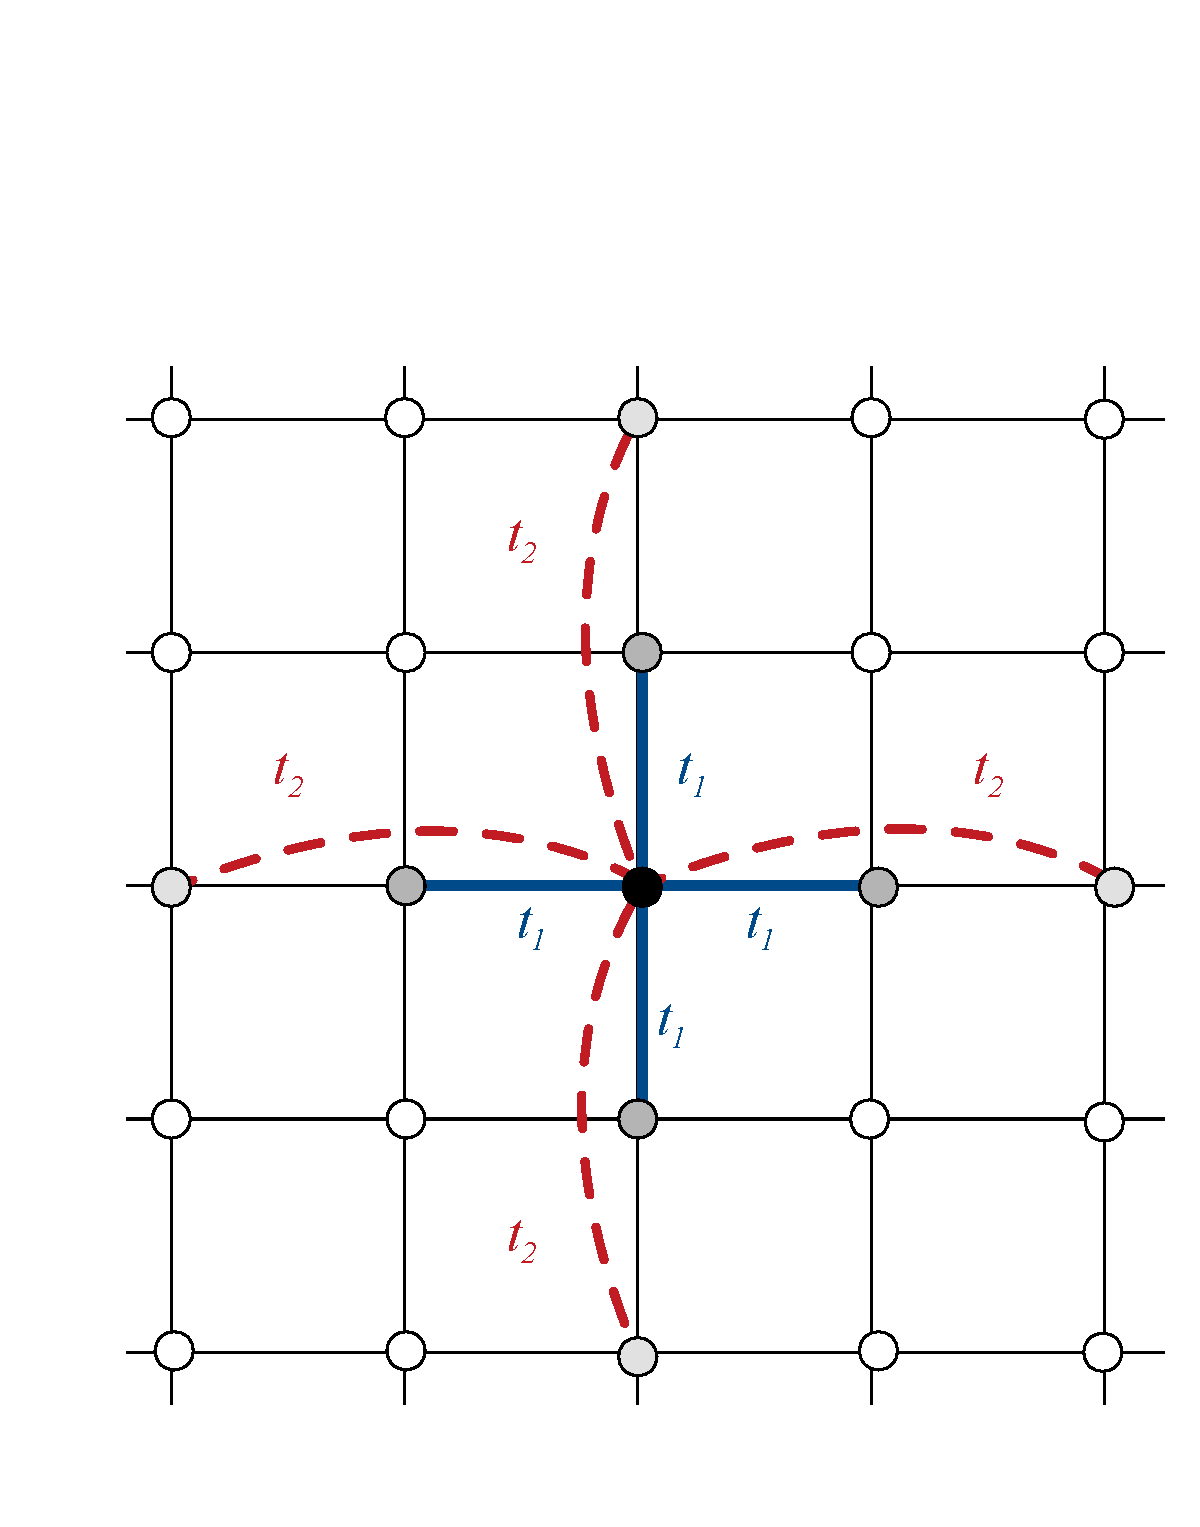
\includegraphics[width=1.5in]{quartic-hofstadter-hoppings-2.pdf}
\caption{\label{hoppings} Nearest-neighbor (NN) and next-nearest-neighbor hopping terms included in the hamiltonian (\ref{quartic-harper}). For the fine-tuned model, we set $t_2 = -t_1/4$.}
\end{figure}

\begin{figure}[thb]
\centering
\hspace{-0.25in}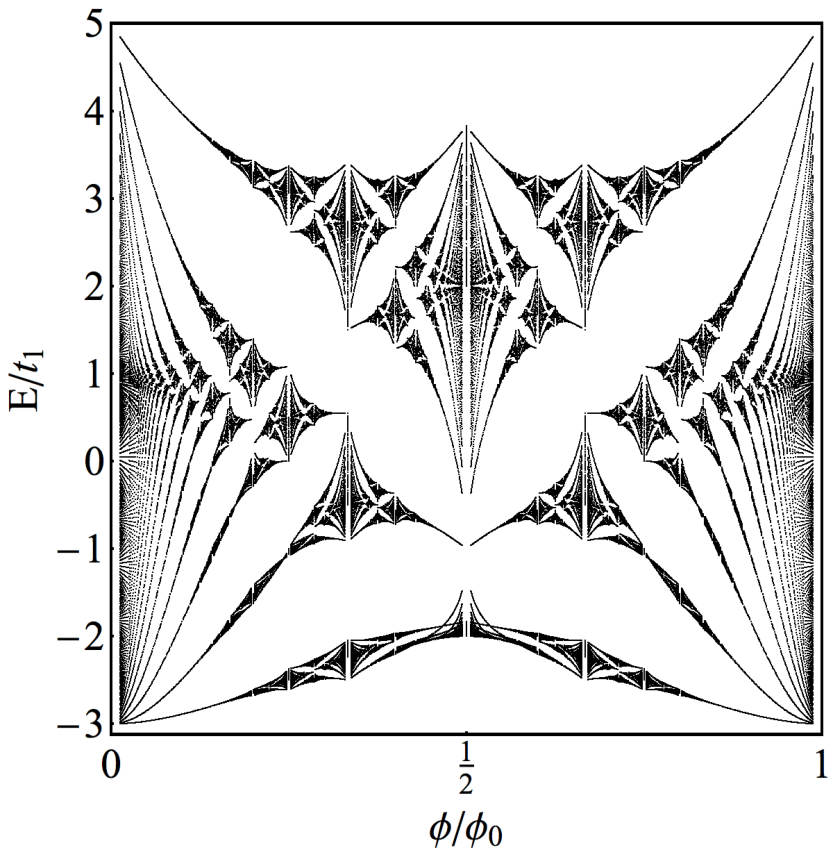
\includegraphics[width=3.1in]{q-butterfly-raster-1200.pdf}
\caption{\label{butterfly-plot} Energy eigenvalues of the lattice Harper-Hofstadter hamiltonian with NNN hoppings (\ref{quartic-harper}) as a function of magnetic flux per elementary lattice plaquette $\phi/\phi_0 = \varepsilon^2/(2\pi) = P/Q$.}
\end{figure}

% \begin{figure}[thb]
% \centering
% 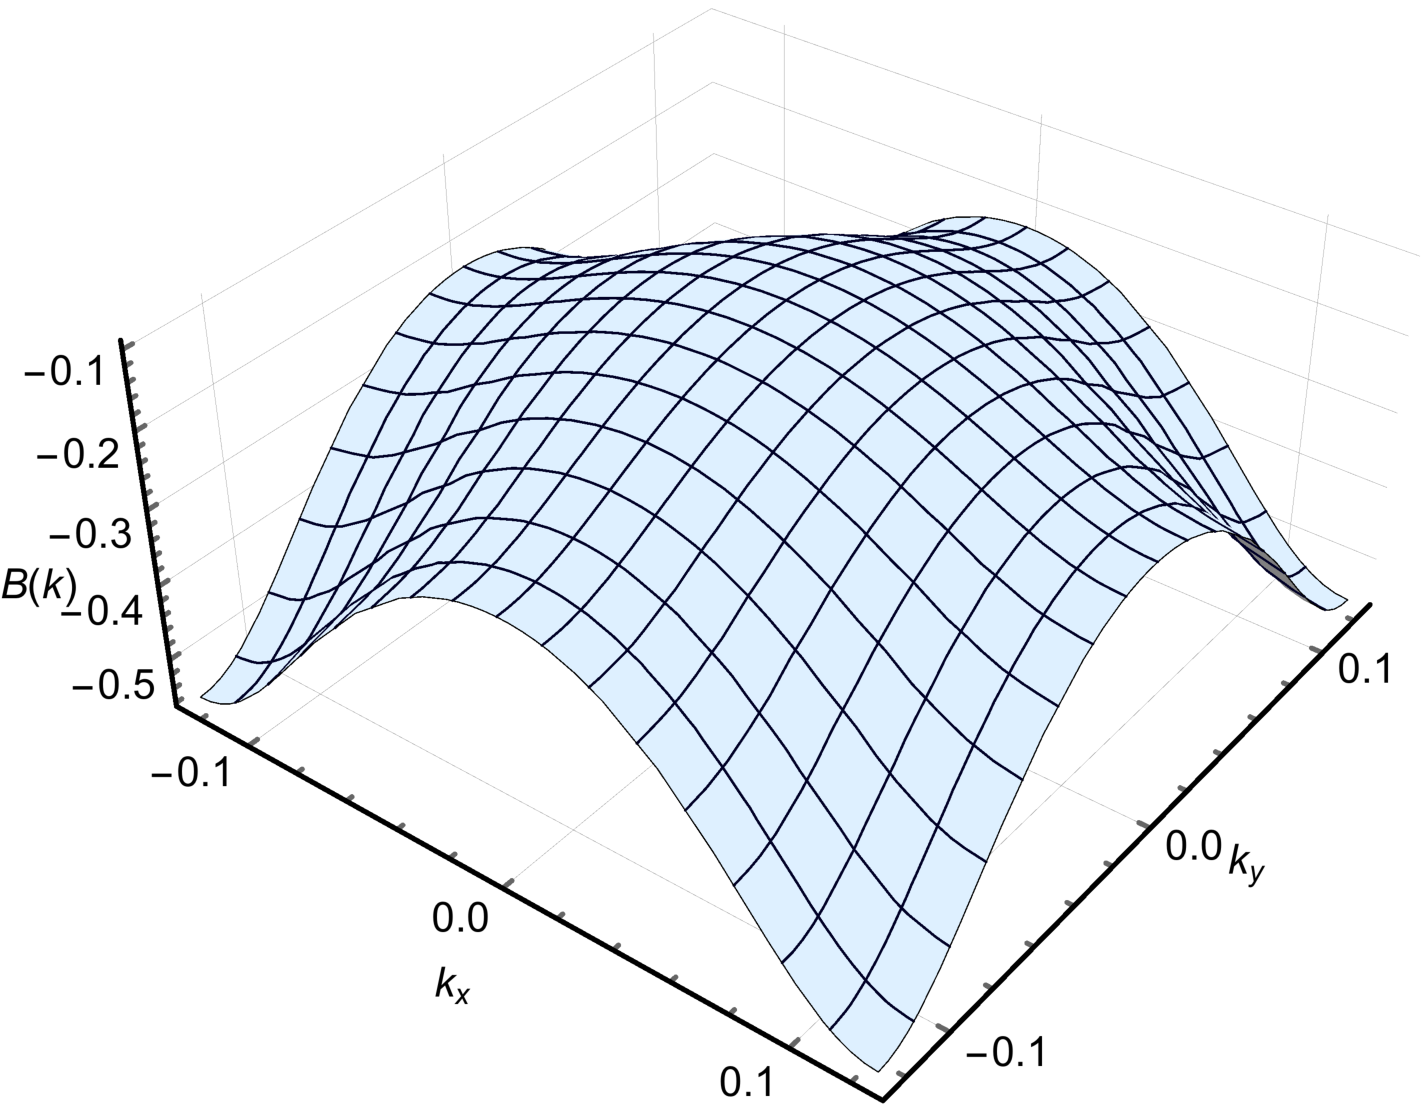
\includegraphics[width=3in]{hof-curvature-2.pdf}
% 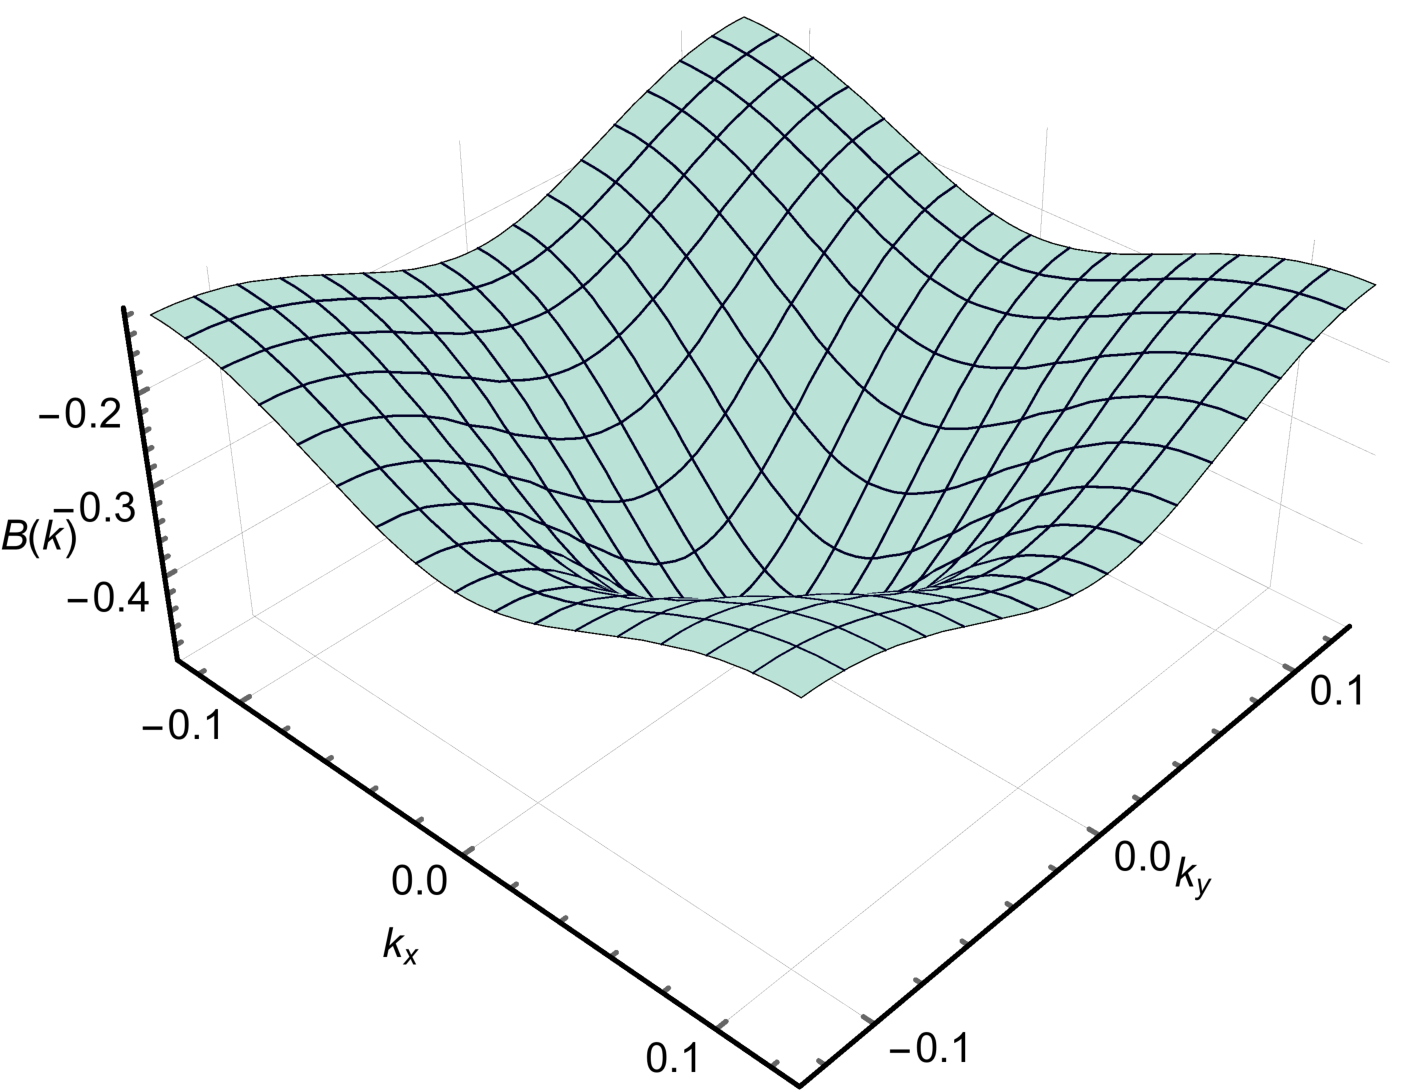
\includegraphics[width=3in]{quartic-curvature-2.pdf}
% \caption{\label{curv-fluctuations} Comparison of fluctuations in Berry curvature $B(\mathbf{k})$ over the magnetic Brillouin zone for the Hofstadter model (top) and the quartic model (\ref{quartic-harper}) (bottom) at the fine-tuned point $t_2 = -t_1/4$. The flux per plaquette in both cases is $\phi/\Phi_0 = 1/4$. The integral of $B(\mathbf{k})$ over the MBZ -- the Chern number -- has magnitude 1 for both bands.}
% \end{figure}

\begin{figure}[thb]
\centering
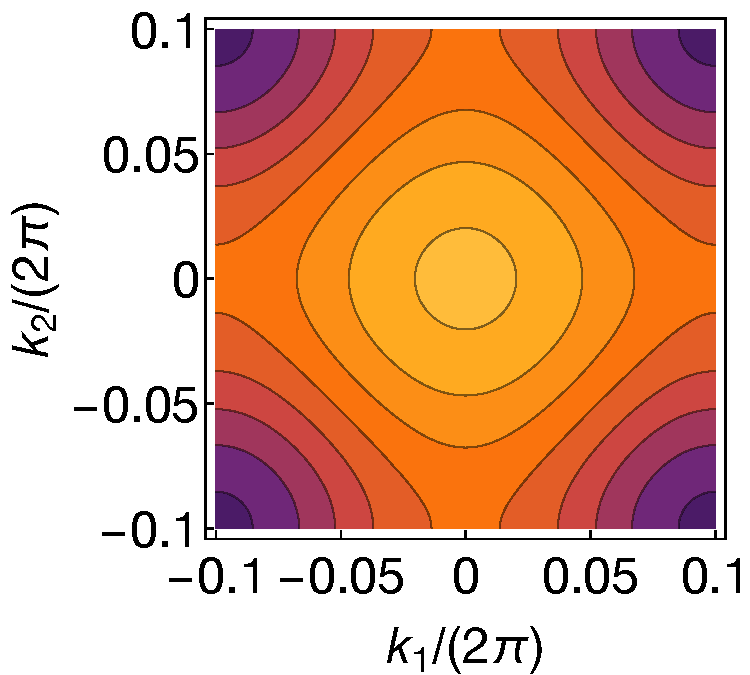
\includegraphics[width=1.4in]{curv-hof-n5.pdf}
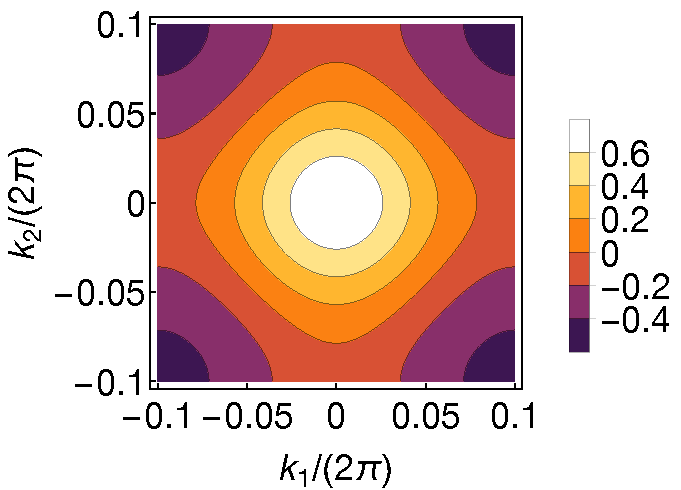
\includegraphics[width=1.75in]{curv-qrt-n5.pdf}
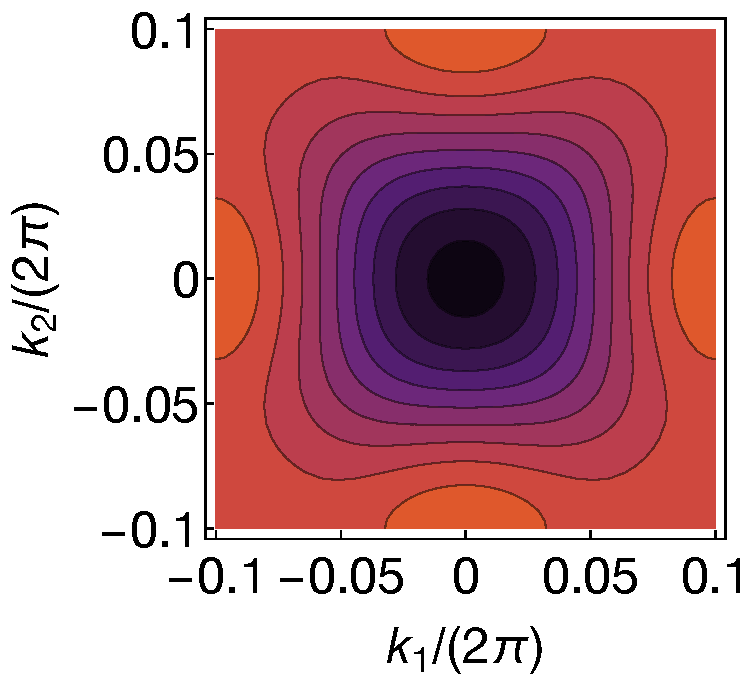
\includegraphics[width=1.4in]{norm-tr-hof-n5.pdf}
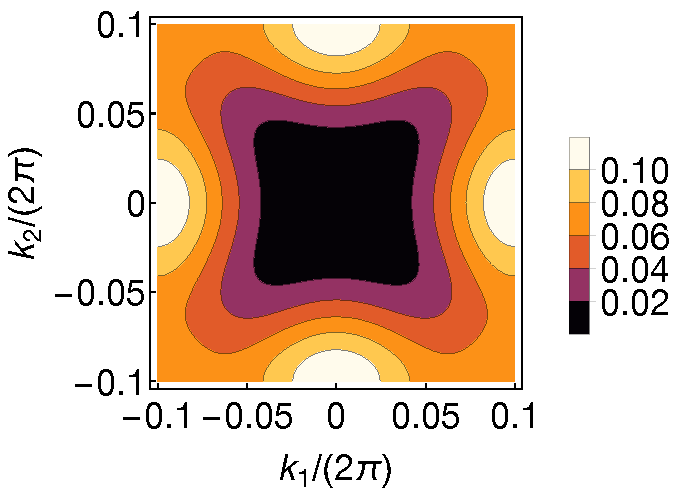
\includegraphics[width=1.75in]{norm-tr-qrt-n5.pdf}
\caption{Comparison of magnetic Brillouin zone geometry between Hofstadter (left) and quartic (right) models at flux per plaquette $\phi/\phi_0=1/5$. The top left panel shows the Berry curavture $B(\mathbf{k})$ for the Hofstadter model; the top right panel shows $B(\mathbf{k})$ for the quartic model. The bottom panels show the normalized trace inequality $\bar{T}(\mathbf{k}$}
\end{figure}

As in Section \ref{landau-level-limit}, we can write this in terms of the hermitian generators of lattice translations,
\begin{align*}
H_0 = &-2t_1\left(\cos(\Pi_1) + \cos(\Pi_2)\right)\\ &- 2t_2\left(\cos(2\Pi_1) + \cos(2\Pi_2)\right)
\end{align*}
Replacing the cosine terms by their Taylor expansion, the terms lowest-order in the momenta are 
\begin{align*}{}
H_0 = &-4 t_1 - 4 t_2 + (t_1 + 4t_2) \left(\Pi_1^2 + \Pi_2^2\right) \\
&- \left(\frac{t_1}{12} + \frac{4}{3}t_2\right) \left(\Pi_1^4 + \Pi_2^4\right) + \ldots
\end{align*}

If we make the particular choice of hopping amplitudes $t_2 = -t_1/4$, then the quadratic terms vanish exactly, and we are left with an effective hamiltonian that is quartic in the momenta to lowest order,
\begin{align}
\label{hamiltonian-quartic-effective}
H_{\text{eff}} = -3t_1 + \frac{t_1}{4} \left(\Pi_1^4 + \Pi_2^4\right).
\end{align}
The negative hopping amplitude could in principle be realized in optical lattice experiments by periodic ``shaking'' of the lattice. Unlike the Landau level hamiltonian, this hamiltonian does not have $SO(2)$ rotational symmetry, but it is symmetric under the square lattice isometry group $D_4$. The particular quartic momentum operator in (\ref{hamiltonian-quartic-effective}) can be written
\begin{align*}
\Pi_1^4 + \Pi_2^4 = \left(\Pi_1^2 + \Pi_2^2\right)^2 - \left(\Pi_1^2\Pi_2^2 + \Pi_2^2\Pi_1^2\right),
\end{align*}
that is, as the square of the Landau-level hamiltonian plus a term that explicitly breaks the rotational symmetry.

As in the Landau level problem, we can choose a gauge and introduce Fock operators $a$, $a^{\dag}$ corresponding to the cyclotron momenta $\Pi_a$. For example, we choose the Landau gauge and the Fock operators
\begin{align*}
a &= \frac{1}{\sqrt{2}\varepsilon}\left(\Pi_1 - i\Pi_2\right),\\
a^{\dag} &= \frac{1}{\sqrt{2}\varepsilon}\left(\Pi_1 + i\Pi_2\right).
\end{align*}
In terms of these operators,
\begin{align*}
\left(\Pi_1^2 + \Pi_2^2\right)^2 &= 4\left(a^{\dag}a + \frac{1}{2}\right)^2 \\
\Pi_1^2\Pi_2^2 + \Pi_2^2\Pi_1^2 &= -\frac{1}{2}\left(a^4 + a^{\dag\,4}\right) + \left(a^{\dag}a + \frac{1}{2}\right)^2 - \frac{3}{4}
\end{align*}

The effective hamiltonian is
\begin{align}
\label{effective-fock-hamiltonian}
H_{\text{eff}} = \frac{t_1\varepsilon^4}{8}\left[a^4 + a^{\dag 4} + 6\left(a^{\dag}a + \frac{1}{2}\right)^2 + \frac{3}{2}\right].
\end{align}

We numerically approximate this hamiltonian by working in a basis of number eiegenstates $\ket{n}$ staisfying $a^{\dag}a{\ket{n}}=n{\ket{n}}$ and truncating to a finite-dimensional subspace. This gives estimates for the cyclotron energies and overlaps with the Landau level states. We find good agreement between this continuum approximation truncated to $n \leq 1000$ and exact numerical energy levels of lattice hamiltonian for small $\varepsilon$. The first two nonzero overlaps of the ground state $\ket{\tilde{0}}$ of the hamiltonian (\ref{effective-fock-hamiltonian}) with the Landau level states are $\braket{\tilde{0}}{0}\approx0.9991$, $\braket{\tilde{0}}{4}\approx-0.0422$. The large overlap with the $\ket{\tilde{0}}$. In terms of Fock operators, the trace inequality takes the particularly simple form $\expval{T} = 2\expval{a^{\dag}a}$\cite{bauer_quantum_2016}. Calculating this in the truncated Landau level basis, we find $\expval{T} \approx0.0143$, in good agreement with the value found from intergrating the lattice $T(\mathbf{k})$ over the MBZ, $\expval{T} \approx 0.0145$.

We can study the spectrum of cyclotron orbits of this hamiltonian semiclassically by applying the Bohr-Sommerfeld quantization condition. In our notation this is
\begin{align*}
\oint\limits_{H=E_n} \Pi_1\, d\Pi_2 = 2\pi n,
\end{align*}
with the integral taken over a closed curve of constant energy in classical phase space. From this condition we find
\begin{align*}
E_n \sim n^2\phi^2, 
\end{align*}
in agreement both with the numerically-obtained, approximate spacing of the cyclotron levels, and with the quadratic dependence of $E$ on $\phi$ observed in the butterfly plot, Fig. \ref{butterfly-plot}.


\subsection{Many-body gap from numerical exact diagonalization}
The bands of our weak-field lattice hamiltonian correspond to cyclotron orbits that are distinct from Landau levels. However, we still expect that fractionally filling these bands with interacting particles will lead to FQH phases. To verify this, we numerically diagonalize a two-body interaction hamiltonian projected to these bands. We consider the bosonic Laughlin state at $\nu = 1/2$ filling, and the fermionic Laughlin state at $\nu = 1/3$. For the bosonic case, we study $N_p=8$ bosons interacting via hard-core repulsion. We use magnetic unit cells of size of various square dimensions $m \times m$ for integral $m$, and a total system size of $4\times4$ MUC. For the fermionic case we use a repulsive nearest-neighbor interaction, and a lattice of $4\times6$ MUC of dimension $3m\times2m$.  We carry out our numerical diagonalization on a torus, and verify that the many-body ground states have the appropriate topological degeneracy for a Laughlin fluid on a torus. For both the Hofstadter model and our quartic model, the dispersion, Berry curvature, and Fubini-Study metric are all uniform over the MBZ up to exponentially small corrections\cite{Harper:2014vi,bauer_quantum_2016}. Geometric stability considerations\cite{jackson_geometric_2015} then suggest that the trace inequality $\expval{T}$ should provide information about the size of the many-body gap.

\subsection{Deviations from fine-tuning}
We now consider small perturbations away from the fine-tuned case $t_2 = -t_1/4$ by seting $t_2 = \left(-\frac{1}{4} + \delta\right)t_1$. In this case, instead of (\ref{hamiltonian-quartic-effective}) above, we have an effective hamiltonian with a quadratic term, ,
\begin{align*}
\label{delta-hamiltonian}
H_{\text{eff}} = t_1 \left[\left(\frac{1}{4}-\frac{4\delta}{3}\right)\left(\Pi_1^4 + \Pi_2^4\right) + 4\delta \left(\Pi_1^2 + \Pi_2^2\right)\right].
\end{align*}
If we make the $\varepsilon$ dependence explicit by rescaling, we have
\begin{align}
H_{\text{eff}} = \frac{t_1\varepsilon^4}{4} \left[\left(1 - \frac{16\delta}{3}\right)\left(P_1^4 + P_2^4\right) + \frac{16\delta}{\varepsilon^2} \left(P_1^2 + P_2^2\right)\right].
\end{align}
For a fixed $\delta$, we can always decrease the external magnetic flux density $B$, hence $\varepsilon$, such that the quadratic term dominates, and our Chern bands are effectively Landau levels. However for a fixed $\varepsilon$, $\delta$ may be small enough that the quadratic term can be treated as a perturbation to the quartic term, with perturbative parameter $16 \delta/\varepsilon^2$ (with both $\varepsilon,\,\delta$ small). A weak upper bound on the range of the small $\delta$ regime is given by enforcing $16 \delta/\varepsilon^2 < 1$ or $\delta < \varepsilon^2/16$. 

% In terms of Fock operators, the hamiltonian (\ref{delta-hamiltonian}) is
% \begin{align*}
% H_{\text{eff}} = \frac{t_1\epsilon^4}{4} \left[\frac{1}{8}\left[a^4 + a^{\dag 4} + 6\left(a^{\dag}a + \frac{1}{2}\right)^2 + \frac{3}{2}\right]. + \frac{16\delta}{\epsilon^2} \left(a^{\dag}a + \frac{1}{2}\right)\right]
% \end{align*}

% Ref. \onlinecite{Aidelsburger:2014hm} observed the Hofstadter model in a system of ultracold atoms in an optical lattice, with effective values of $\epsilon^2 = 2\pi/4$ and $t_1 = (75\pm3\text{s}^{-1})2\pi \hbar$. 

% Numerical evidence suggests that the weak-field regime sets near $\phi/\Phi_0 \approx 1/15$, as measured by convergence of band-geometric quantities to their asymptotic values\cite{Bauer2016}.

While we introduced $\delta$ to parameterize perturbations from our fine-tuned model, we could also view $\delta$ as a tunable parameter in its own right. In particular, varying $\delta$ between $0$ and $1/4$ interpolates between our quartic model ($\delta=0$) and the Hofstadter model($\delta=1/4$). We numerically calculate the value of the trace inequality of this model $\expval{T}$ for a few $\delta$ in the interval  , and plot the results in Fig. (\ref{trace-delta-plot}). 

\begin{figure}[thb]
\centering
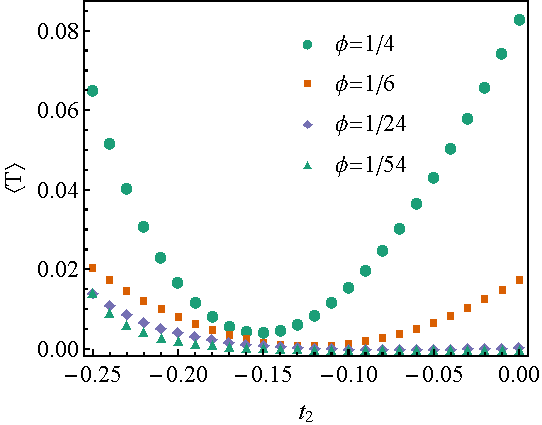
\includegraphics[width=3.0in]{trace-delta-plot-new.pdf}
\caption{\label{trace-delta-plot}}
\end{figure}

\begin{figure}[thb]
\centering
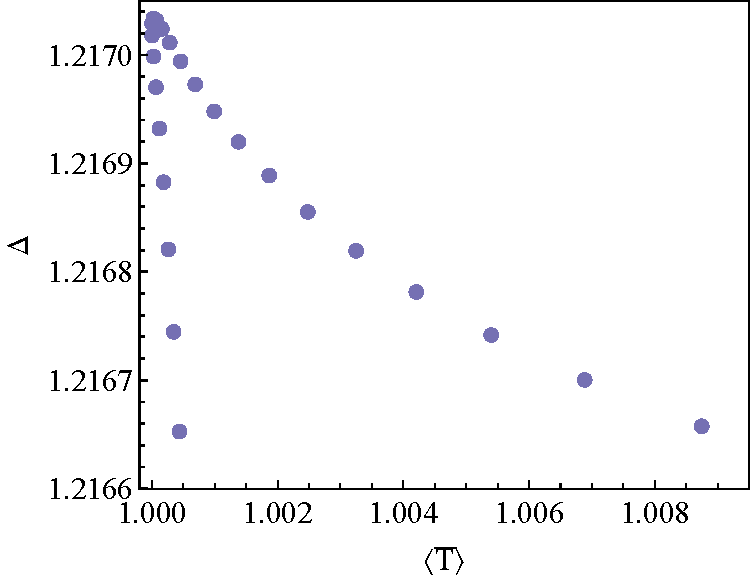
\includegraphics[width=3.0in]{gap-v-trace-delta.pdf}
\caption{\label{gap-v-trace-delta-plot}Many-body gap of $N_p=8$ interacting fermions at $\nu=1/3 $filling the lowest band of the quartic model (\ref{quartic-harper}). In this plot, $\phi/\phi_0=1/24$, and the fermions interact via a repulsive next-nearest neighbor potential. We }
\end{figure}

\section{Generalizations}
Although the previous section focused on a particular choice of hopping parameters, it is clear that in priciple one can engineer arbitrary inversion-symmetric band structures. The most general such model, following the discussion in Sec. \ref{landau-levels} is
\begin{align*}
H_{\text{eff}} = \sum_{j,k}t_{jk}\left(\Pi_1^{j}\Pi_2^{k} + \Pi_2^{k}\Pi_1^{j}\right)
\end{align*}

To quartic order in the lattice translation generators, we have
\begin{align}
\label{general-quartic}
H_{\text{eff}} = h_{ab}\Pi_a \Pi_b + \lambda_{abcd} \Pi_a \Pi_b \Pi_c \Pi_d + \ldots.
\end{align}
where the coefficient tensors $h_{ab}$, $\lambda_{abcd}$ are completely symmetric in their indicies. 


If we consider the Hofstadter model with all next-nearest-neighbor (NNN) hopping terms, including the hopping diagonally across a plaquette, we obtain
\begin{align*}
H_0 = &-t_1 \left(\widetilde{T}_1 + \widetilde{T}_2\right)\nonumber - t_2 \left(\widetilde{T}_1^{2} + \widetilde{T}_2^{2}\right)\\ &- t_3 \left(\widetilde{T}_1\widetilde{T}_2 + \widetilde{T}_2 \widetilde{T}_1\right) + \text{h.c.}
\end{align*}

We can write this in terms of the generators $\Pi_a$ as
\begin{align*}
H_0 = &-2t_1 \left[\cos\left(\Pi_1\right) + \cos\left(\Pi_2\right)\right]\\ &-2t_2 \left[\cos\left(2\Pi_1\right)+\cos\left(2\Pi_2\right)\right]\\ &- 4t_3 \cosh\left(\frac{\epsilon^2}{2}\right)\cos\left(\Pi_1 + \Pi_2\right).
\end{align*}

Expanding to quartic order, we obtain the low-$\epsilon$ effective hamiltonian
\begin{align*}
H_{\text{eff}} = h_{ab}\Pi_a \Pi_b + \lambda_{abcd} \Pi_a \Pi_b \Pi_c \Pi_d 
\end{align*}

with coefficients

\begin{align*}
h_{11} = h_{22} &= t_1 + 4t_2 + 2t_3,\\
h_{12} &= 2t_3,
\end{align*}
and 
% \begin{align*}
% \lambda_{1111} &= \lambda_{2222} = -\frac{1}{3}\left(t_1/4 + 4t_2 + t_3/2\right)
% \lambda_{1112}  &= \lambda_{1222} = -t_3/3\\
% \lambda_{1122} &= -t_3/2
% \begin{align*}
\begin{align*}
\lambda_{1111} = \lambda_{2222} &= -\frac{1}{3}\left(\frac{t_1}{4} + 4t_2 + \frac{t_3}{2} \right),\\
\lambda_{1112}  = \lambda_{1222} &= -t_3/3,\\
\lambda_{1122} &= -t_3/2.
\end{align*}


% Consider just the quadratic part of this hamiltonian,
% \begin{align*}
% H_0 = h_{ab}\Pi_a \Pi_b
% \end{align*} We would like to choose Fock operators such that $H_0 = \frac{\omega}{2}\left(a^{\dag}a + aa^{\dag}\right).$ One way to implement this map would be to first perform a coordinate transformation on the momentum phase space that diagonalizes the effective mass tensor $h_{ab}$, then introduce Fock operators in, e.g. the Landau gauge in terms of the new momenta. A second way to do this is to forgoe the coordinate transformation and explicitly choose Fock operators that bring $H_0$ into this form.

% A choice of Fock operators is equivalent to a choice of positive complex structure on $\mathbf{R}^2$ compatible with the symplectic form on $\mathbf{R}^2$. A generic choice of such a complex structure is equivalent to a choice of $\tau \in \mathbf{H}$, with $\mathbf{H} = \left\{\tau \in \mathbf{C}, \text{Im}\,\tau >0\right\}$ the complex upper half-plane, and yields Fock operators
% \begin{align*}
% a = \frac{1}{\sqrt{2\tau_2}\epsilon}\left(\Pi_1 - \tau\Pi_2\right)\\
% a^{\dag} = \frac{1}{\sqrt{2\tau_2}\epsilon}\left(\Pi - \tau^{\ast}\Pi_2\right).
% \end{align*}

% In order to put our hamiltonian to take the form $H_0 = \omega\left(a^{\dag}a + aa^{\dag}\right)/2$, we choose
% \begin{align*}
% \tau = \frac{1}{h_{11}}\left(\sqrt{|h|} - i h_{12}\right).
% \end{align*}
% where $|h| = \text{det}\,h = \omega^2/(4\varepsilon^4).$


\section{Conclusion}
We have constructed a Harper-Hofstadter model with cyclotron orbits that are distinct from Landau levels in the continuum limit. This provides a regime in which to study the quantum Hall effect that is distinct from both the Landau level 2DEG and FCI models. 

One drawback of our numerical approach is that we diagonalize the many-body interaction hamiltonian on a lattice, and as pointed out in Ref., this explicit symmetry breaking may induce spurious gaps in Goldstone modes. Other numerical methods 


\begin{acknowledgments}
The authors thank Tom Jackson for collaboration on related work and for his band geometry code. We also thank authors of the DiagHam package, which was used in this work.

\end{acknowledgments}
\bibliographystyle{apsrev4-1}
\bibliography{landau-orbits}
%\bibliography{quartic-zotero/quartic-zotero}

\clearpage
% \appendix
% \section{Quartic hamiltonian effective hamiltonian for $C_4$ symmetric NNN hoppings.}
% In this section, we consider the Hofstadter model with all next-nearest-neighbor (NNN) hopping terms -- including the hopping diagonally across a plaquette and find the effective quartic hamiltonian. The hoppings are selected to preserve the underlying $C_4$ symmetry of the lattice. Specifically, we choose 
% \begin{align*}
% H_0 = &-t_1 \left(\widetilde{T}_1 + \widetilde{T}_2\right)\nonumber - t_2 \left(\widetilde{T}_1^{2} + \widetilde{T}_2^{2}\right)\\ &- t_3 \left(\widetilde{T}_1\widetilde{T}_2 + \widetilde{T}_2 \widetilde{T}_1\right) + \text{h.c.}
% \end{align*}

% We can write this in terms of the generators $\Pi_a$ as
% \begin{align*}
% H_0 = &-2t_1 \left[\cos\left(\Pi_1\right) + \cos\left(\Pi_2\right)\right]\\ &-2t_2 \left[\cos\left(2\Pi_1\right)+\cos\left(2\Pi_2\right)\right]\\ &- 4t_3 \cosh\left(\frac{\epsilon^2}{2}\right)\cos\left(\Pi_1 + \Pi_2\right).
% \end{align*}

% Expanding to quartic order, we obtain the low-$\epsilon$ effective hamiltonian
% \begin{align*}
% H_{\text{eff}} = h_{ab}\Pi_a \Pi_b + \lambda_{abcd} \Pi_a \Pi_b \Pi_c \Pi_d 
% \end{align*}

% with coefficients

% \begin{align*}
% h_{11} = h_{22} &= t_1 + 4t_2 + 2t_3,\\
% h_{12} &= 2t_3,
% \end{align*}
% and 
% % \begin{align*}
% % \lambda_{1111} &= \lambda_{2222} = -\frac{1}{3}\left(t_1/4 + 4t_2 + t_3/2\right)
% % \lambda_{1112}  &= \lambda_{1222} = -t_3/3\\
% % \lambda_{1122} &= -t_3/2
% % \begin{align*}
% \begin{align*}
% \lambda_{1111} = \lambda_{2222} &= -\frac{1}{3}\left(\frac{t_1}{4} + 4t_2 + \frac{t_3}{2} \right),\\
% \lambda_{1112}  = \lambda_{1222} &= -t_3/3,\\
% \lambda_{1122} &= -t_3/2.
% \end{align*}


\end{document}


